\section{Objective}

This project investigates techniques for producing 3d models using consumer
grade depth sensors. The goal is to use the Intel RealSense D435 camera (the D435),
the Software Development Kit (the RealSense SDK) and the Viewer to capture
depth images and point clouds.

State of the art techniques pioneered by Kinect Fusion \cite{newcombe2011kinectfusion}
 build models incrementally by merging (or fusing) a series of depth images into
 a common frame of reference. These techniques require careful memory management,
 shared data structures enabling fast searches and parallel programming to exploit
 graphics processors.

In order to better understand these techniques, I simulate the algorithm by
manually collecting, cleaning and merging point clouds, then attempting
to reconstruct polygonal meshes. I have dubbed my two reconstruction projects
Cube Man and Joe Head.

\begin{figure}[h]
 \centering
 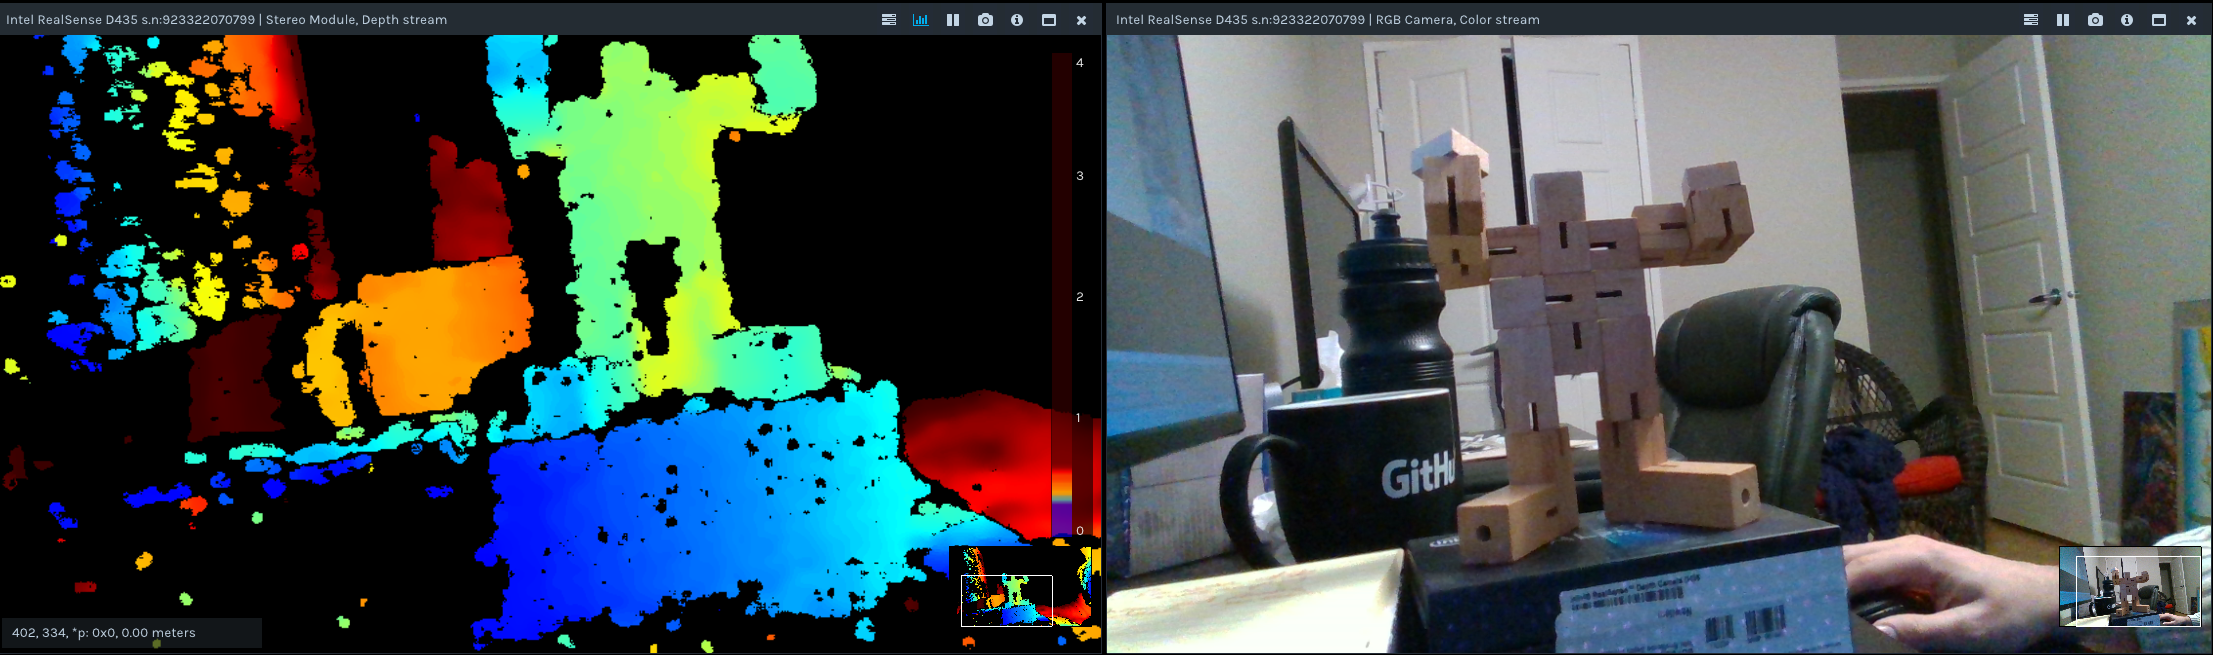
\includegraphics[width=0.75\textwidth]{cube_man_selfie.png}
\caption{Project Cube Man}
\end{figure}

\begin{figure}[h]
\centering
 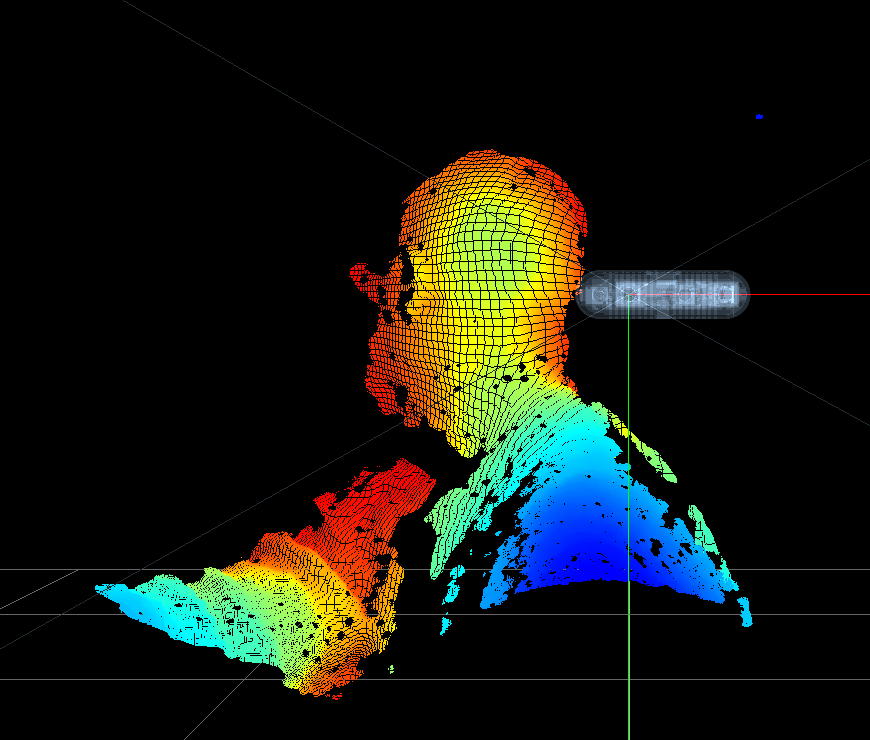
\includegraphics[width=0.45\textwidth]{snapshot_back_of_head.png}
  \caption{Project Joe Head}
 \end{figure}
